\documentclass[a4paper, 14pt]{extarticle}
\usepackage[russian]{babel}
\usepackage[T1]{fontenc}
\usepackage{fontspec}
\usepackage{indentfirst}
\usepackage{enumitem}
\usepackage{graphicx}
\usepackage[
  left=20mm,
  right=10mm,
  top=20mm,
  bottom=20mm
]{geometry}
\usepackage{parskip}
\usepackage{titlesec}
\usepackage{xurl}
\usepackage{hyperref}
\usepackage{float}
\usepackage[
  figurename=Рисунок,
  labelsep=endash,
]{caption}
\usepackage[outputdir=build, newfloat]{minted}

\hypersetup{
  colorlinks=true,
  linkcolor=black,
  filecolor=blue,
  urlcolor=blue,
}

\renewcommand*{\labelitemi}{---}
\setmainfont{Times New Roman}
\setmonofont{JetBrains Mono}[
  SizeFeatures={Size=11},
]

\newenvironment{code}{\captionsetup{type=listing}}{}
\SetupFloatingEnvironment{listing}{name=Листинг}

\setminted{
  fontsize=\footnotesize,
  frame=lines,
  framesep=2mm,
}

\setlength{\parskip}{6pt}

\setlength{\parindent}{1cm}
\setlist[itemize]{itemsep=0em,topsep=0em,parsep=0em,partopsep=0em,leftmargin=2.0cm,wide}
\setlist[enumerate]{itemsep=0em,topsep=0em,parsep=0em,partopsep=0em,leftmargin=2.0cm,wide}

\renewcommand{\thesection}{\arabic{section}.}
\renewcommand{\thesubsection}{\thesection\arabic{subsection}.}
\renewcommand{\thesubsubsection}{\thesubsection\arabic{subsubsection}.}

\titleformat{\section}{\normalfont\bfseries}{\thesection}{0.5em}{}
\titleformat{\subsection}{\normalfont\bfseries}{\thesubsection}{0.5em}{}

\titleformat*{\section}{\normalfont\bfseries}
\titleformat*{\subsection}{\normalfont\bfseries}

\linespread{1.5}
\renewcommand{\baselinestretch}{1.5}

\begin{document}

\begin{titlepage}
  \vspace{0pt plus2fill}
  \noindent

  \vspace{0pt plus6fill}
  \begin{center}
    Санкт-Петербургский национальный исследовательский университет
    информационных технологий, механики и оптики

    \vspace{0pt plus3fill}

    Факультет инфокоммуникационных технологий

    Направление подготовки 11.03.02

    \vspace{0pt plus2fill}

    Лабораторная работа №2

    <<Разработка серверного web-приложения прикладного назначения>>

  \end{center}

  \vspace{0pt plus6fill}
  \begin{flushright}
    Выполнил: \\
    Швалов Даниил Андреевич

    Группа: К33211

    Проверила: \\
    Марченко Елена Вадимовна
  \end{flushright}

  \vspace{0pt plus5fill}
  \begin{center}
    Санкт-Петербург

    2024
  \end{center}
\end{titlepage}

\section{Введение}

\textbf{Цель работы}: разработать серверное веб-приложение, отвечающее далее
описанным требованиям.

К разрабатываемому приложению предъявляются следующие требования:
\begin{itemize}
  \item серверная часть приложения должна быть реализована с помощью языка
  программирования PHP;
  \item данные должны храниться в СУБД;
  \item структура базы данных должна отвечать правилам нормализации и принципам
  целостности данных в реляционных базах данных.
\end{itemize}

Средствами PHP должны быть программно реализованы следующие функции:
\begin{itemize}
  \item обработка каждого элемента HTML-формы;
  \item загрузка на сервер файлов из HTML-формы и вывод их содержимого на
  страницы сайта;
  \item организация обмена данными с СУБД.
\end{itemize}

Требования к организации базы данных:
\begin{itemize}
  \item БД должна быть реализована средствами любой СУБД, в отчете наличие
  обоснования студентом использования выбранных СУБД;
  \item структура (схема) БД должна состоять минимум из 5 таблиц;
  \item каждая таблица должна соответствовать третьей нормальной форме (3NF);
  \item общая структура (схема) БД должна отвечать правилам поддержания
  целостности данных.
\end{itemize}

\newpage

\section{Ход работы}

В качестве разрабатываемого веб-приложения было выбрано приложение с блогами и
постами, имеющее рабочее название <<Bloggy>>. Оно является аналогом таких
известных сайтов как Habr или Medium. В данном веб-приложении пользователь может
создавать один или несколько блогов. Для каждого блога владелец может создавать
посты. К постам любой пользователь может оставить комментарий или поставить
лайк. Все действия по созданию требуют от пользователя быть авторизованным в
системе. При этом, если пользователь не авторизован, он может просматривать
блоги и посты блогов без ограничений.

Для реализации веб-приложения был выбран язык программирования PHP, а также
фреймворк Symfony. Фреймворк Symfony был выбран поскольку он позволяет вести
быструю разработку и управление веб-приложениями, а также позволяет легко решать
рутинные задачи веб-программиста. Кроме того, он имеет поддержку множества баз
данных (MySQL, PostgreSQL, SQLite или любая другая PDO-совместимая СУБД). У
Symfony большое сообщество и огромное количество документации, а также он
бесплатен и публикуется под лицензией MIT. Это позволяет без проблем
использовать его в учебных проектах.

Для хранения данных приложения была выбрана СУБД PostgreSQL. Данная СУБД
поддерживается в языке программирования PHP и не требует дополнительной
установки внешних библиотек для работы с СУБД. Кроме того, СУБД PostgreSQL
является высокопроизводительным решением, обладающим активным сообществом,
большим количеством документации. Данное решение используется множеством
компаний, поскольку оно зарекомендовало себя как надежное и эффективное
хранилище данных.

На рисунке \ref{fig:puml/database.png} изображена схема таблиц базы данных. На
ней представлены такие таблицы как <<user\_account>>, <<blog>>, <<post>>,
<<comment>> и <<like>>. Описание каждой из этих таблиц представлено ниже.

\begin{figure}[H]
  \centering
  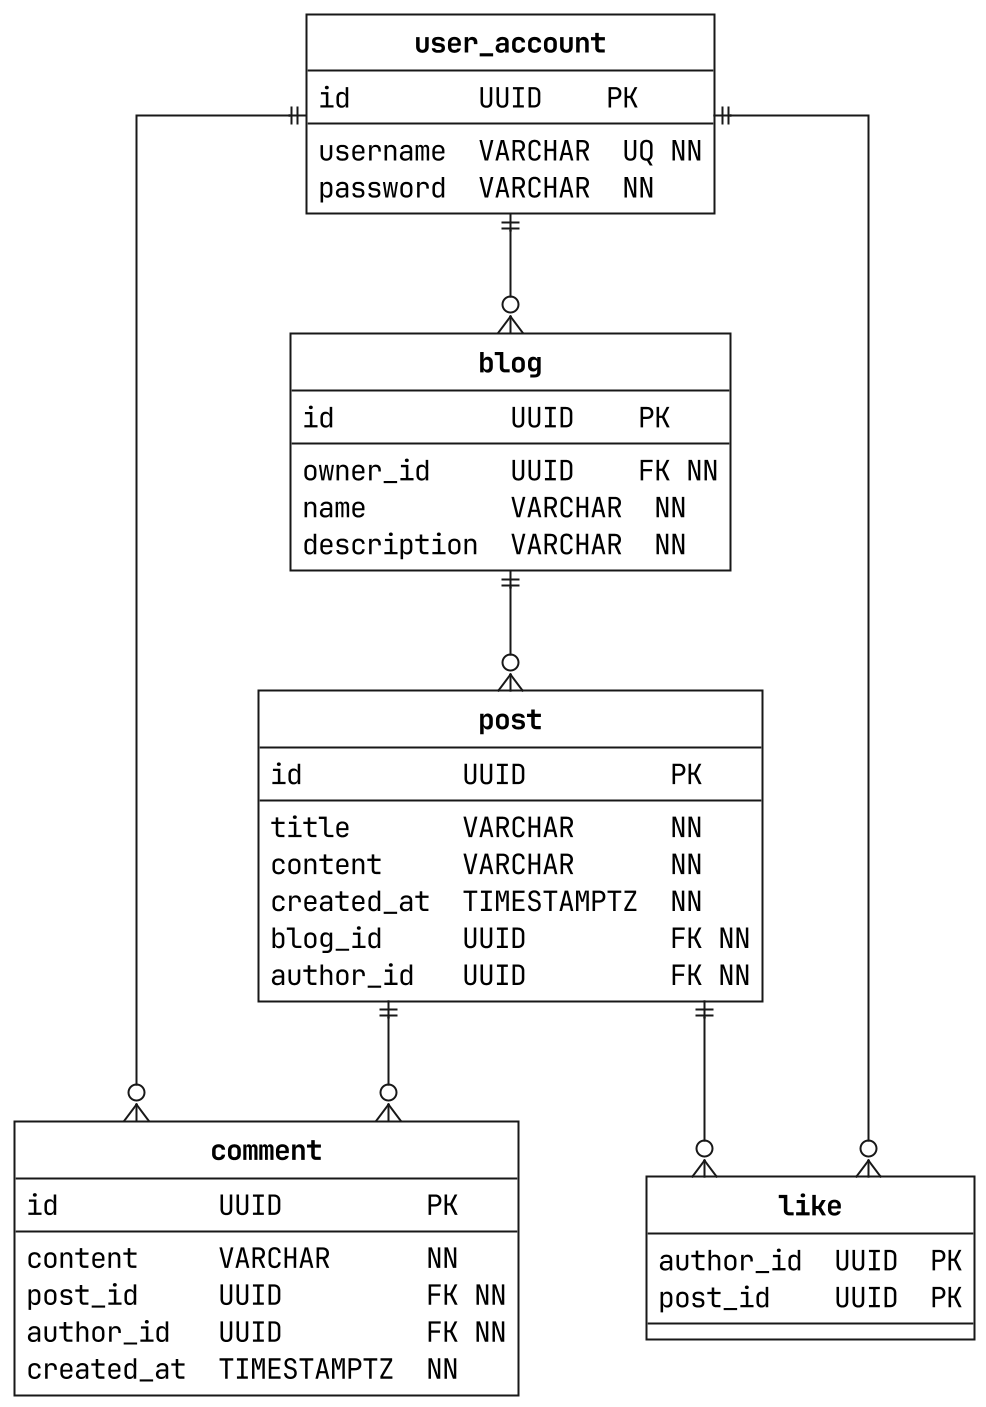
\includegraphics[width=0.6\textwidth]{images/puml/database.png}
  \caption{Схема таблиц базы данных}
  \label{fig:puml/database.png}
\end{figure}

В таблице <<user\_account>> хранится минимально необходимая информация о
пользователе: его идентификатор, имя пользователя и пароль. Они используются для
идентификации и авторизации пользователя.

В таблице <<blog>> хранится информация о блогах: название блога, его описание, а
также идентификатор пользователя, который создал и владеет этим блогом.

В таблице <<post>> хранится информация о каждом посте. Здесь представлена такая
информация, как заголовок и содержимое поста, дата создания, идентификатор
блога, а также идентификатор пользователя, который создал этот пост.

В таблице <<comment>> хранится информация о комментариях: содержимое
комментария, идентификатор поста, к которому относится данный комментарий,
идентификатор автора, а также дата создания.

В таблице <<like>> хранится минимально необходимая информация о лайках постов.
Так, в ней есть идентификатор пользователя, который поставил лайк, а также
идентификатор поста, на который поставили лайк.

При открытии главной страницы веб-приложения пользователю отображается страница,
изображенная на рисунке \ref{fig:blogs.png}. На ней показываются все блоги,
которые существуют в системе. Для просмотра постов блога пользователь может
нажать кнопку <<Перейти>>. Для создания своего блога используется кнопка
<<Создать блог>>.

\begin{figure}[H]
  \centering
  \fbox{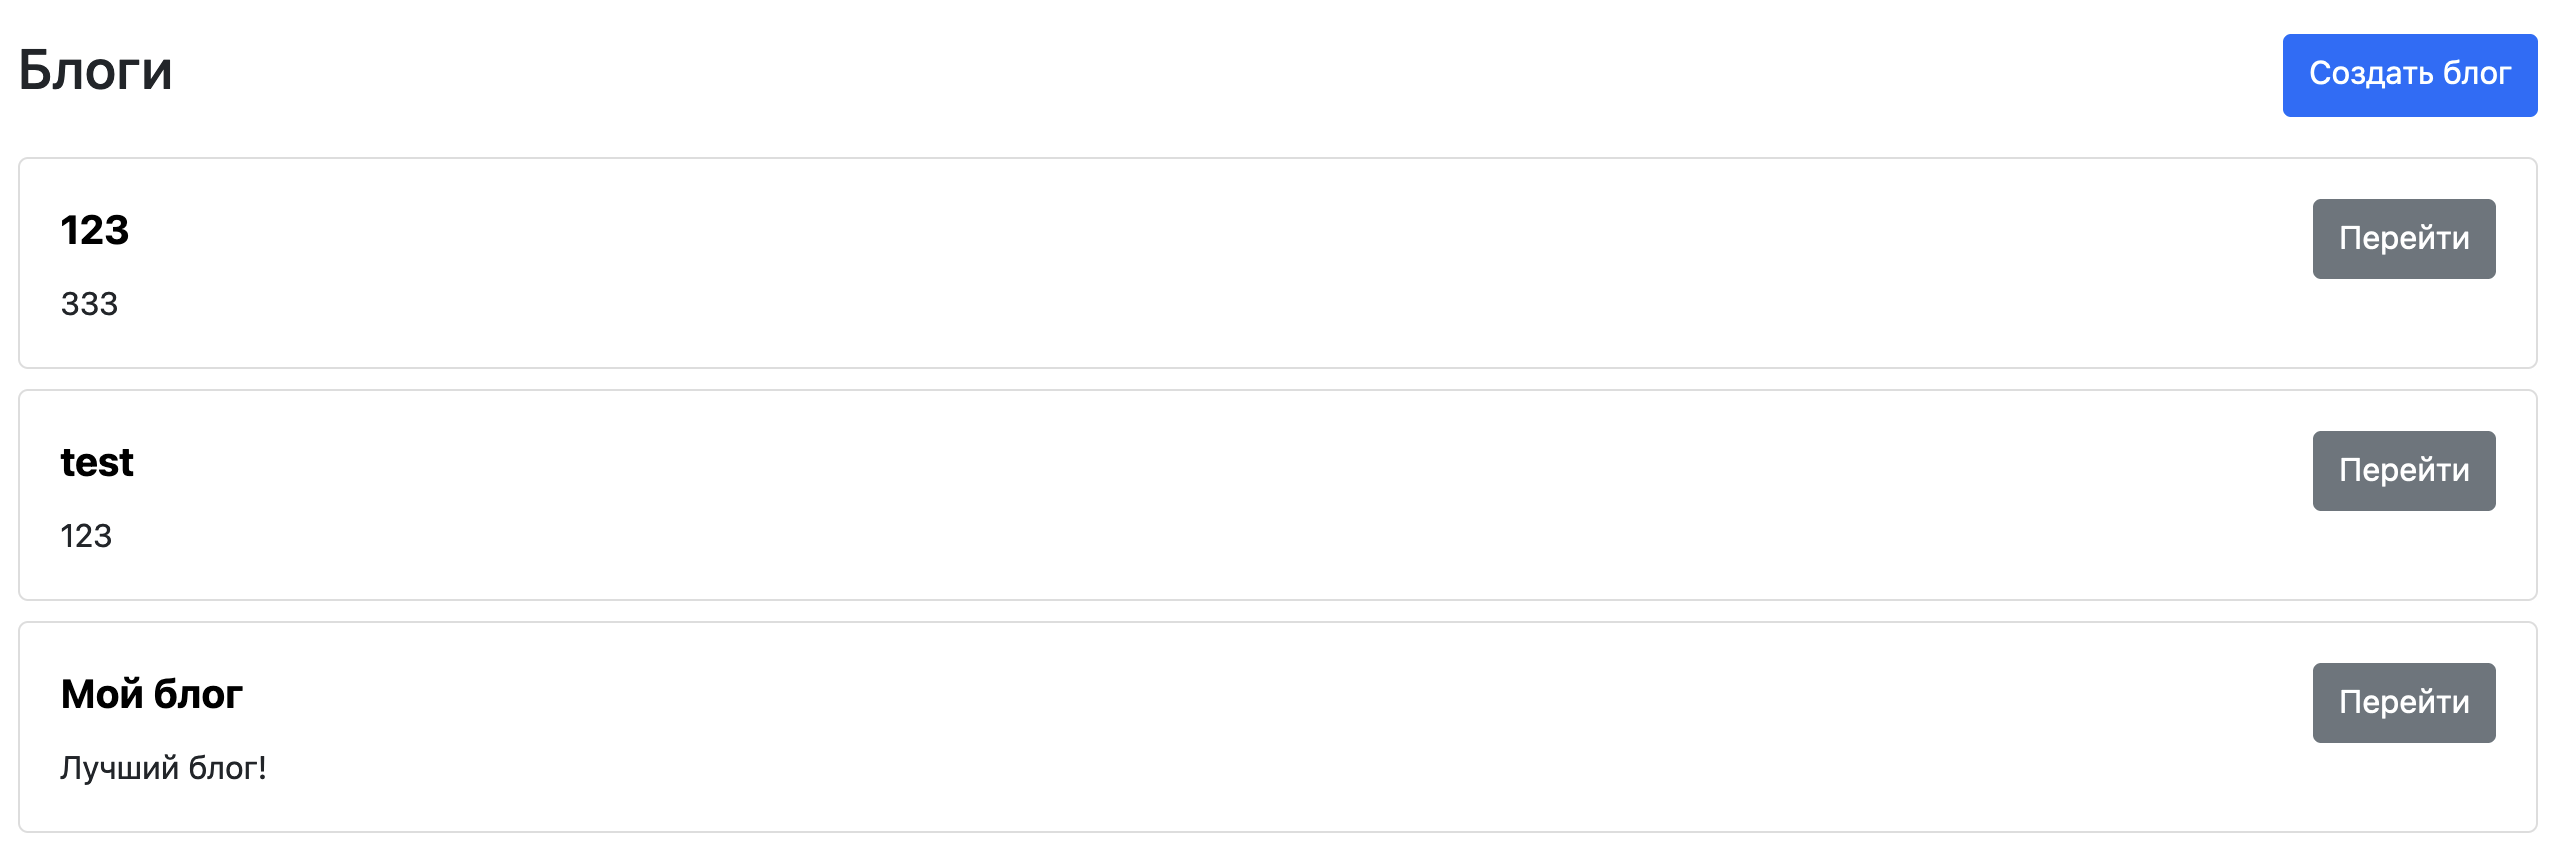
\includegraphics[width=\textwidth]{images/blogs.png}}
  \caption{Страница с блогами}
  \label{fig:blogs.png}
\end{figure}

Для создания блога пользователю нужно быть авторизованным в системе. Поэтому,
если пользователь нажмет на кнопку <<Создать блог>>, при этом будучи
неавторизованным, то его перекинет на страницу входа в аккаунт, которая показана
на рисунке \ref{fig:login.png}.

\begin{figure}[H]
  \centering
  \fbox{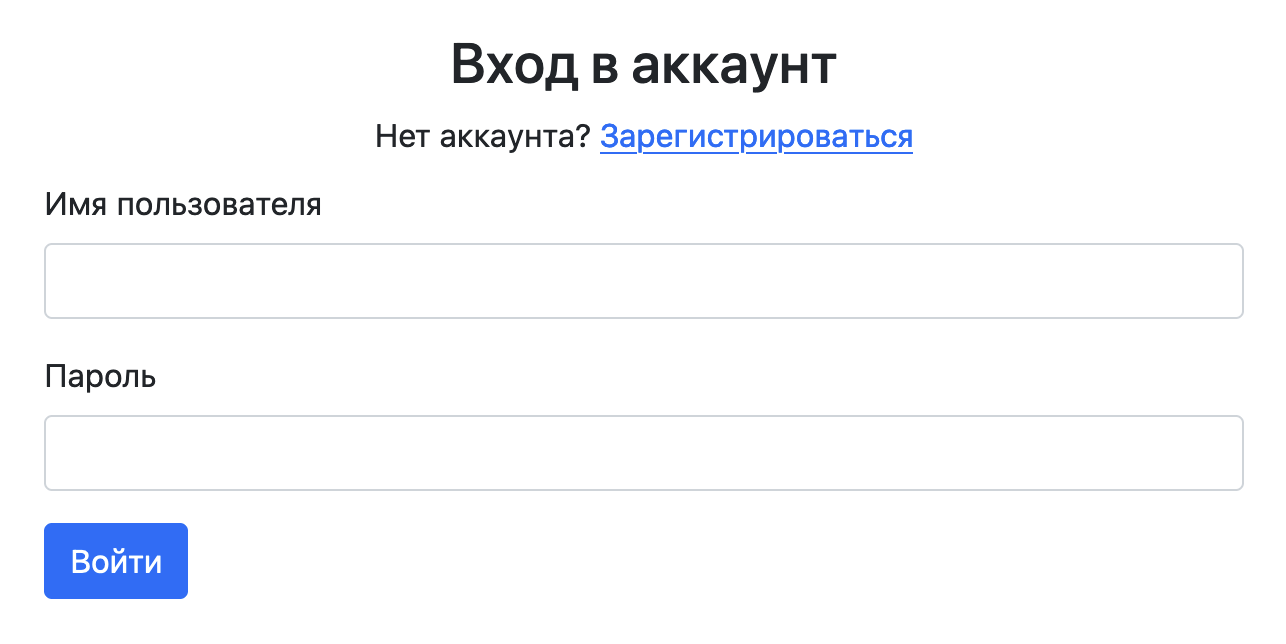
\includegraphics[width=0.7\textwidth]{images/login.png}}
  \caption{Страница входа в аккаунт}
  \label{fig:login.png}
\end{figure}

Если у пользователя еще нет аккаунта в системе, то пользователь может нажать
кнопку <<Зарегистрироваться>>, после чего его перекинет на страницу регистрации,
показанную на рисунке \ref{fig:register.png}.

\begin{figure}[H]
  \centering
  \fbox{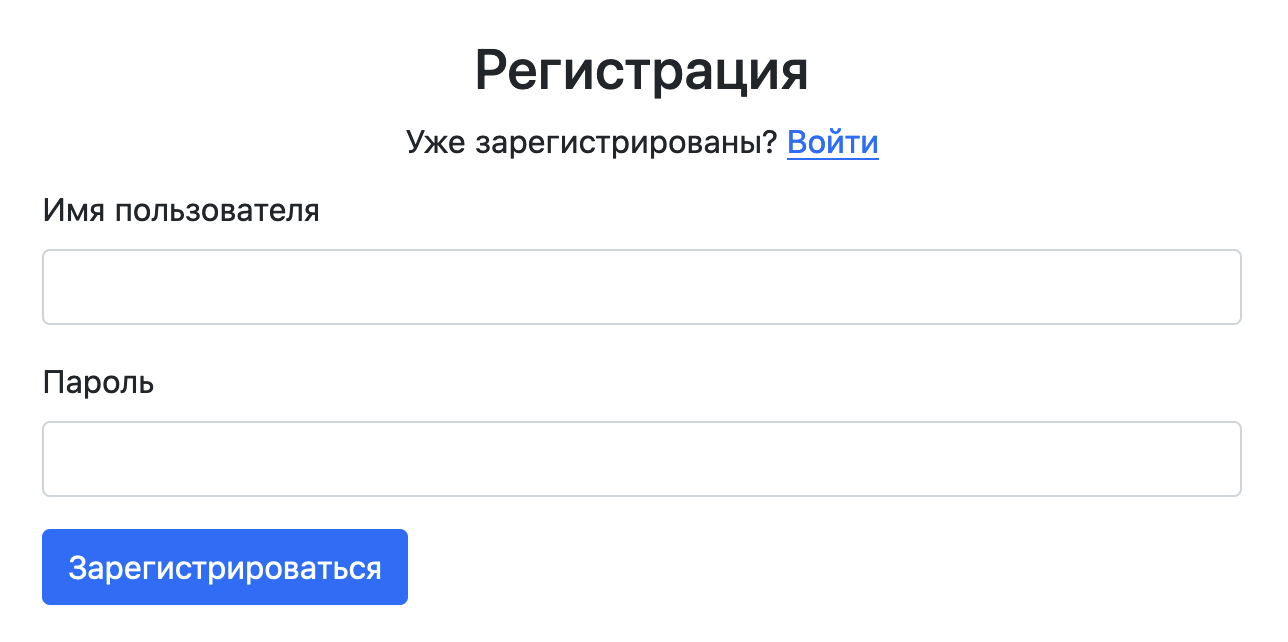
\includegraphics[width=0.7\textwidth]{images/register.png}}
  \caption{Страница регистрации аккаунта}
  \label{fig:register.png}
\end{figure}

Если пользователь был авторизован и нажал на кнопку <<Создать блог>>, то его
перекинет на страницу, изображенную на рисунке \ref{fig:create-blog.png}. На ней
пользователь должен указать название и описание блога. После успешной обработки
формы в базе данных создается новая запись с информацией о блоге.

\begin{figure}[H]
  \centering
  \fbox{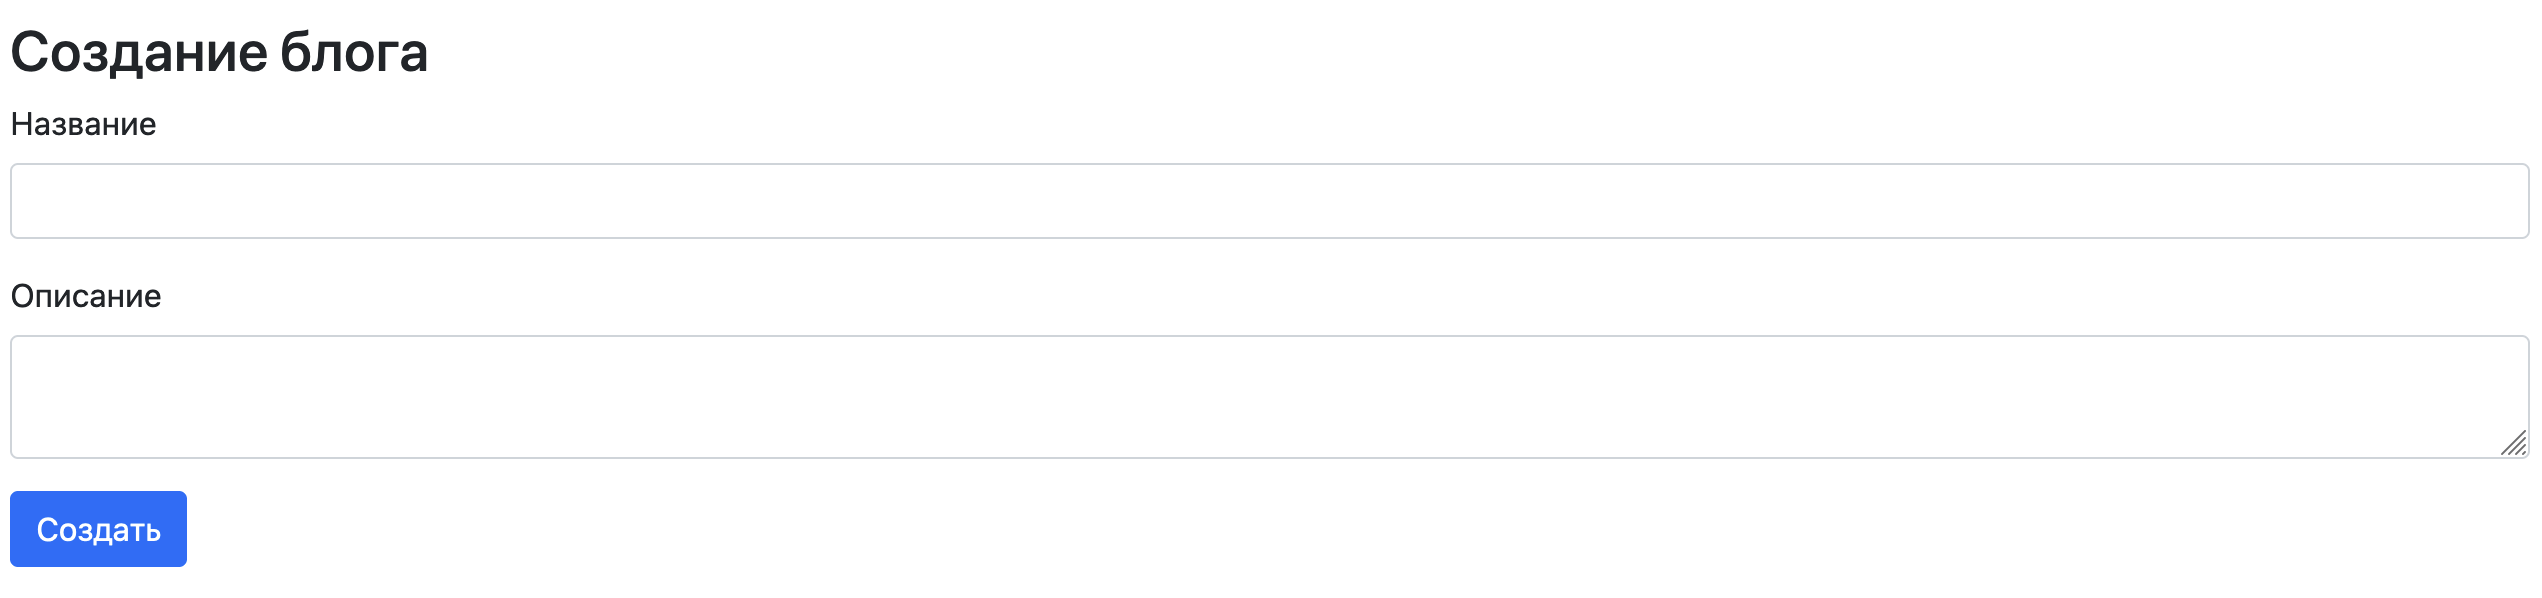
\includegraphics[width=\textwidth]{images/create-blog.png}}
  \caption{Страница создания блога}
  \label{fig:create-blog.png}
\end{figure}

При выборе определенного блога пользователю отображается страница, изображенная
на рисунке \ref{fig:blog.png}. На ней показываются посты, относящиеся к данному
блогу, в порядке убывания даты создания (от самых новых к самым старым). Если
пользователь является владельцем данного блога, то ему также показывается кнопка
<<Создать пост>>. Для каждого поста показывается кнопка <<Перейти>>, которая
позволяет открыть определенный пост для просмотра его содержимого.

\begin{figure}[H]
  \centering
  \fbox{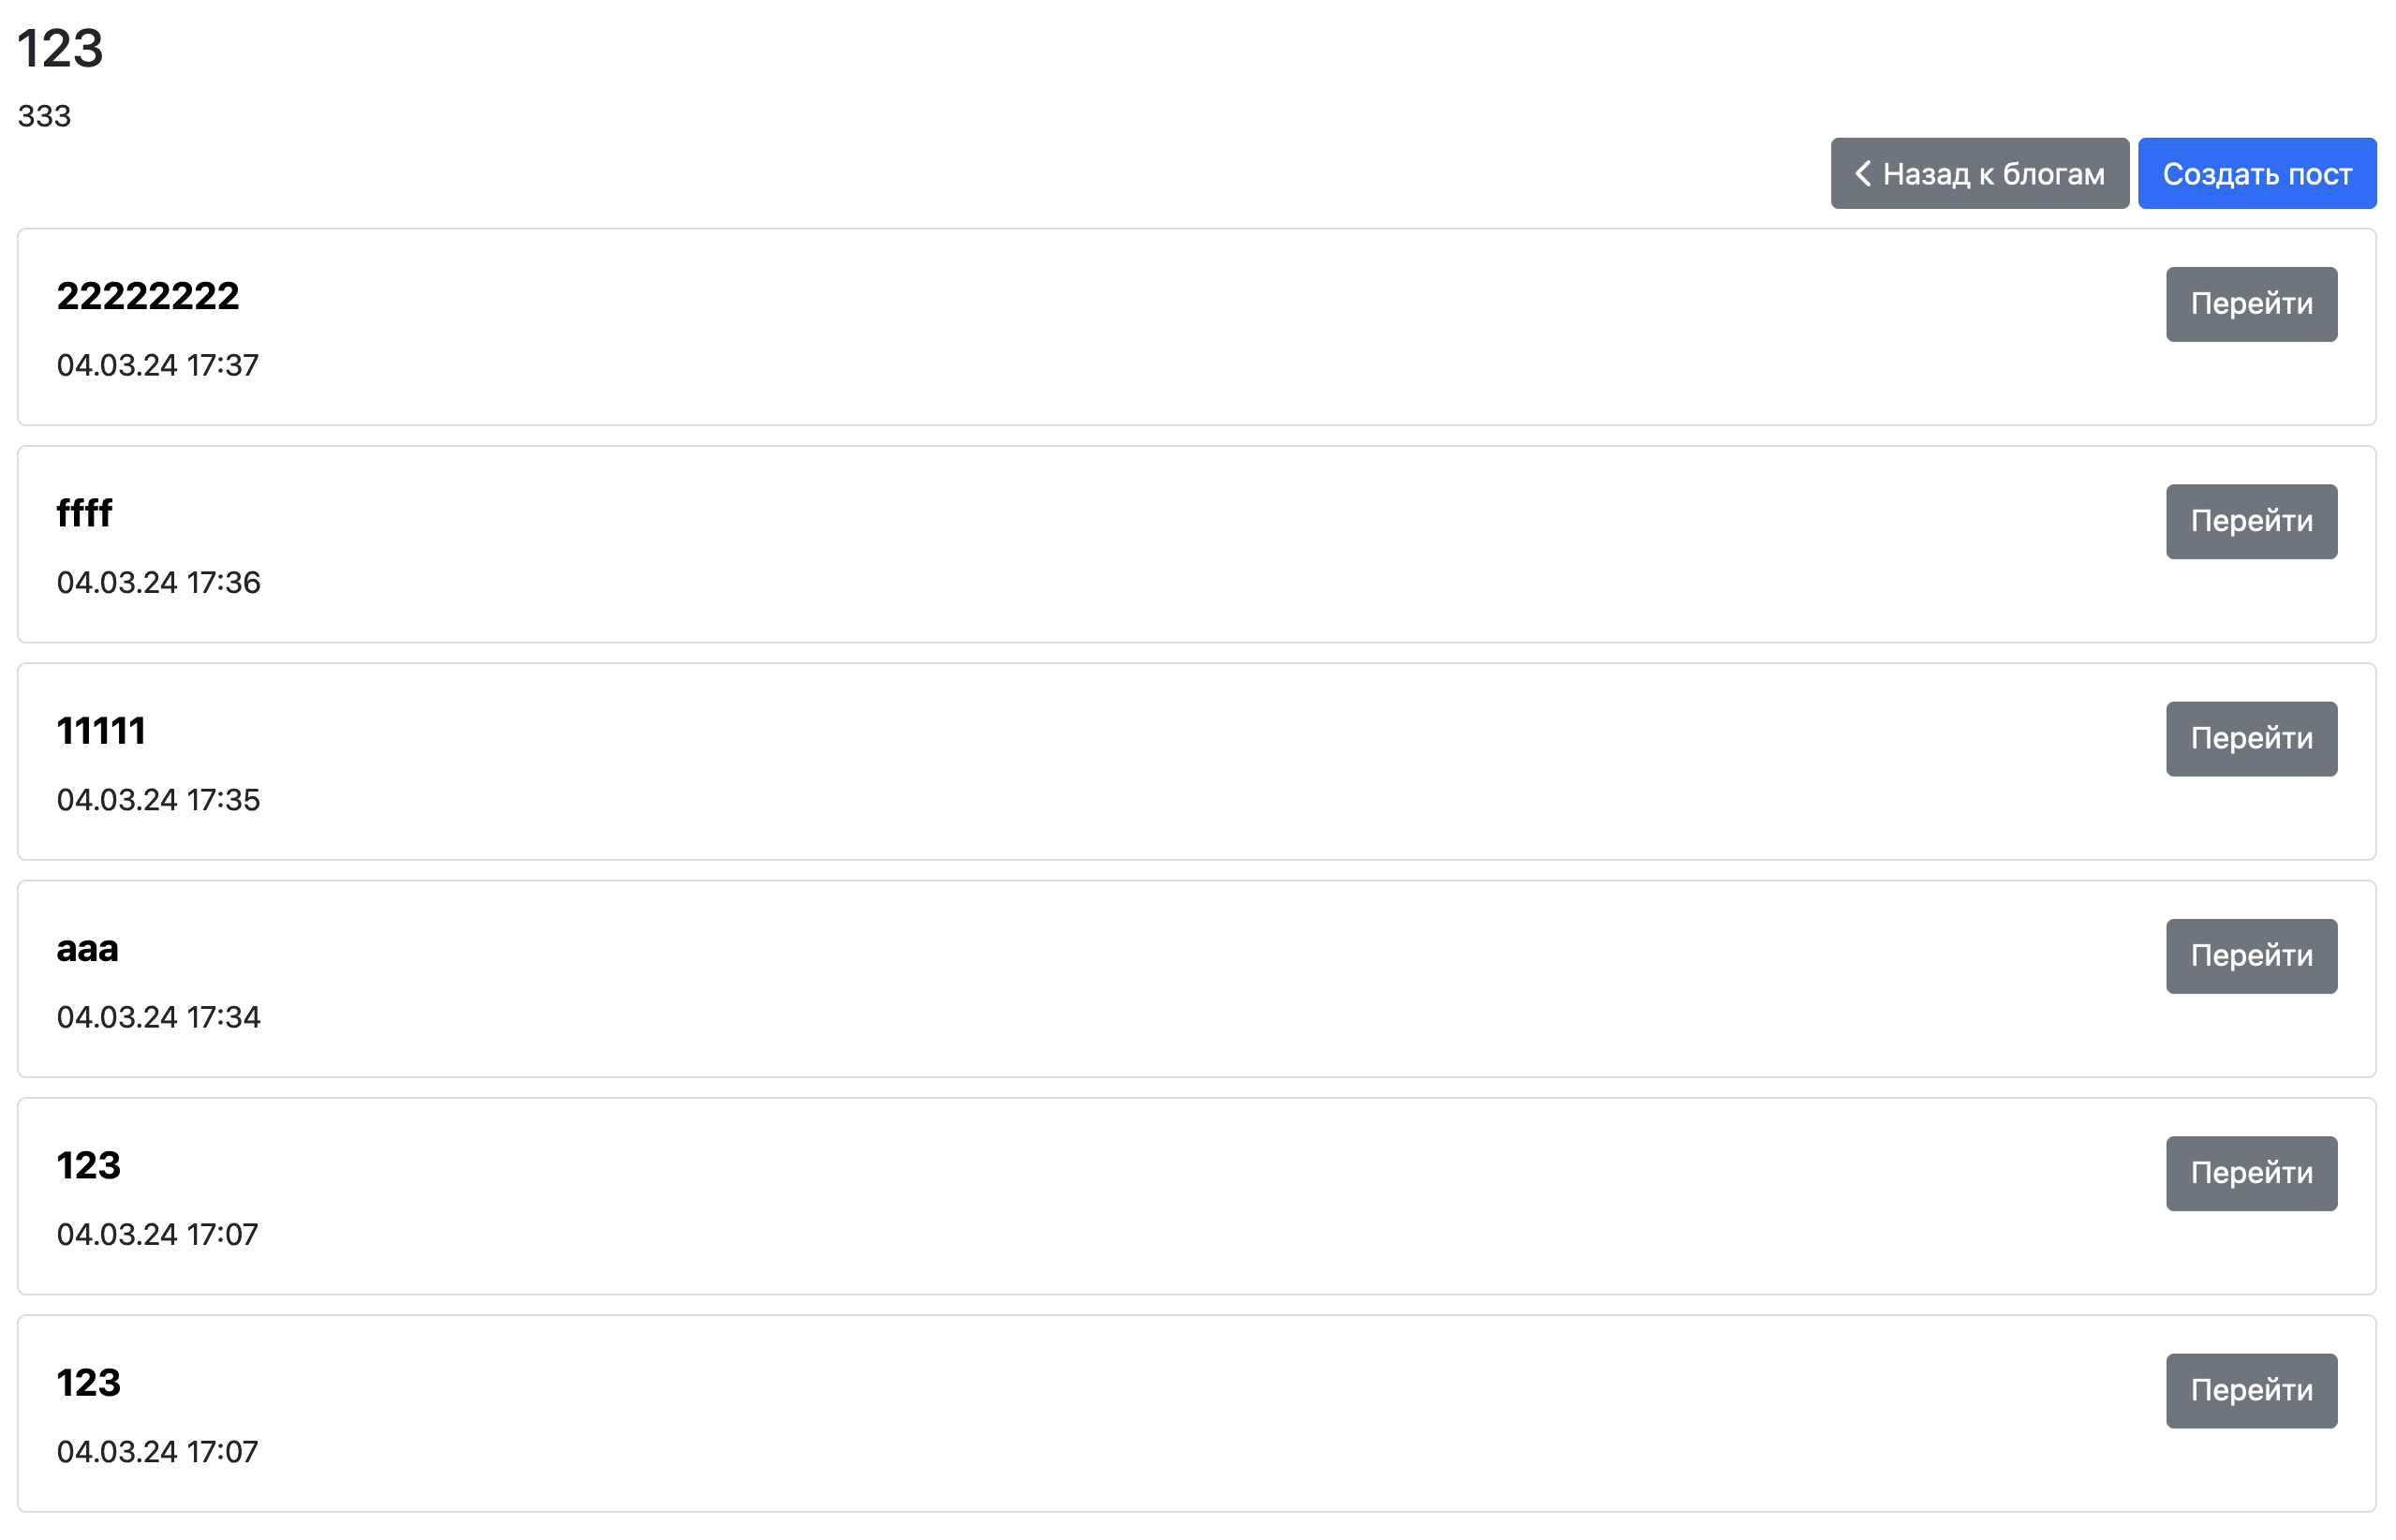
\includegraphics[width=\textwidth]{images/blog.png}}
  \caption{Страница, отображаемая при выборе определенного блога}
  \label{fig:blog.png}
\end{figure}

При нажатии кнопки <<Создать пост>>, пользователю открывается страница,
показанная на рисунке \ref{fig:create-post.png}. На ней пользователю
предлагается ввести заголовок, а также содержимое поста. После успешной
обработки формы эти данные сохраняются в базу данных и пользователя перекидывает
на страницу только что созданного поста.

\begin{figure}[H]
  \centering
  \fbox{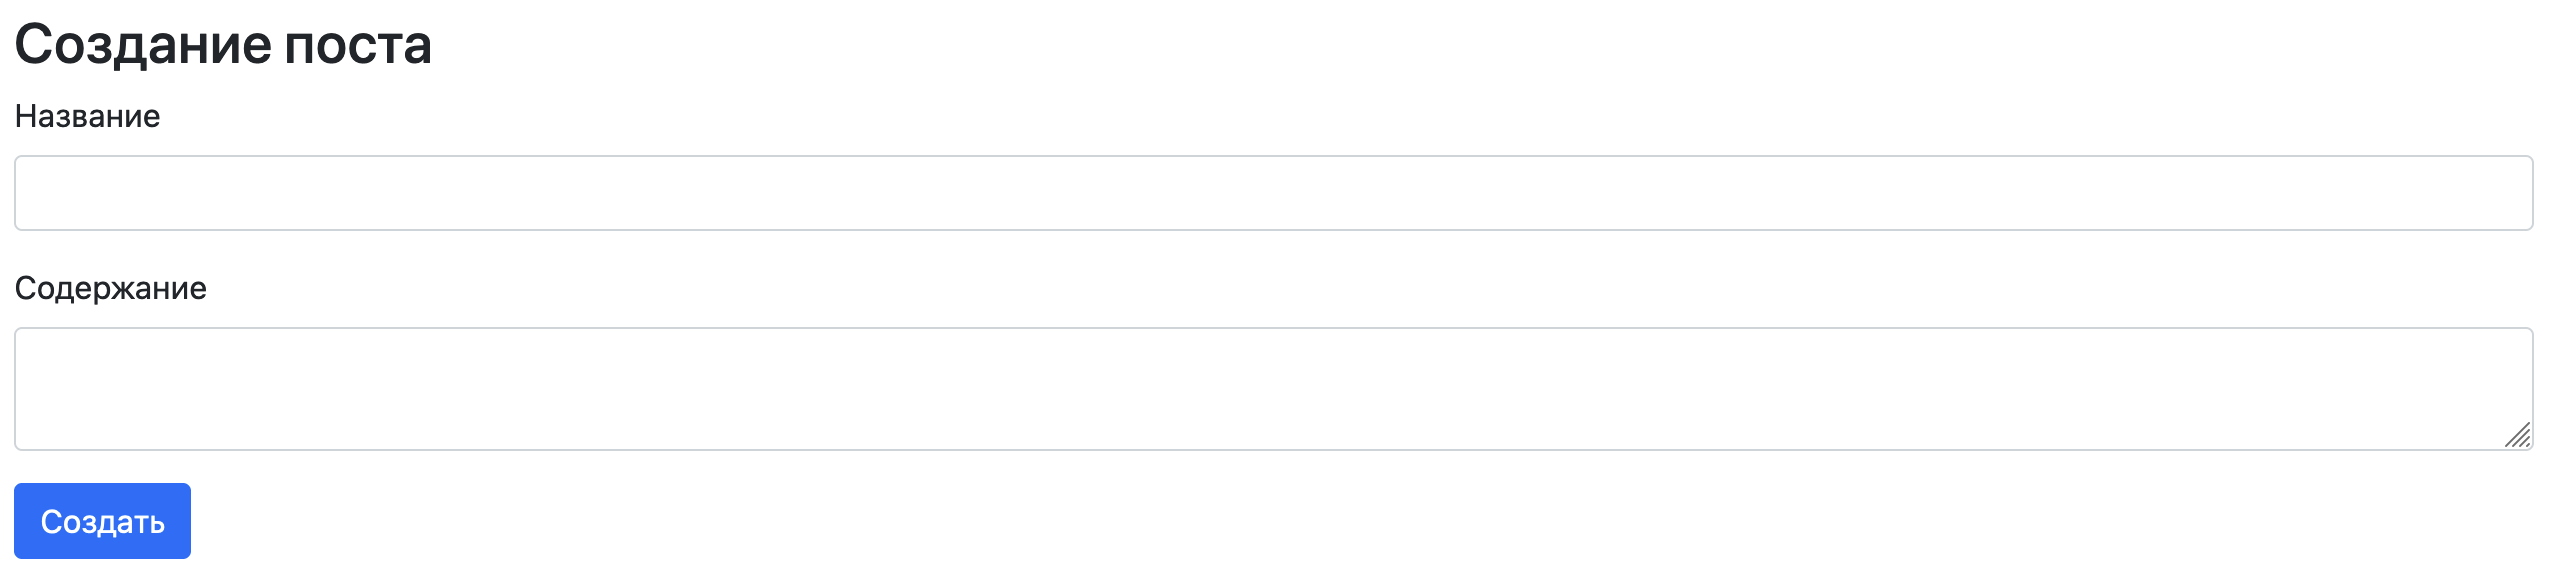
\includegraphics[width=\textwidth]{images/create-post.png}}
  \caption{Страница создания поста}
  \label{fig:create-post.png}
\end{figure}

На рисунке \ref{fig:post.png} показан пример страницы с постом. На ней
пользователь видит заголовок, содержимое, а также дату создания поста. Кроме
того, на данный пост, если пользователь авторизован, можно поставить лайк. Этот
лайк будет сохранен в базе данных. В добавок ко всему, у пользователя есть
возможность оставить комментарий к данному посту.

\begin{figure}[H]
  \centering
  \fbox{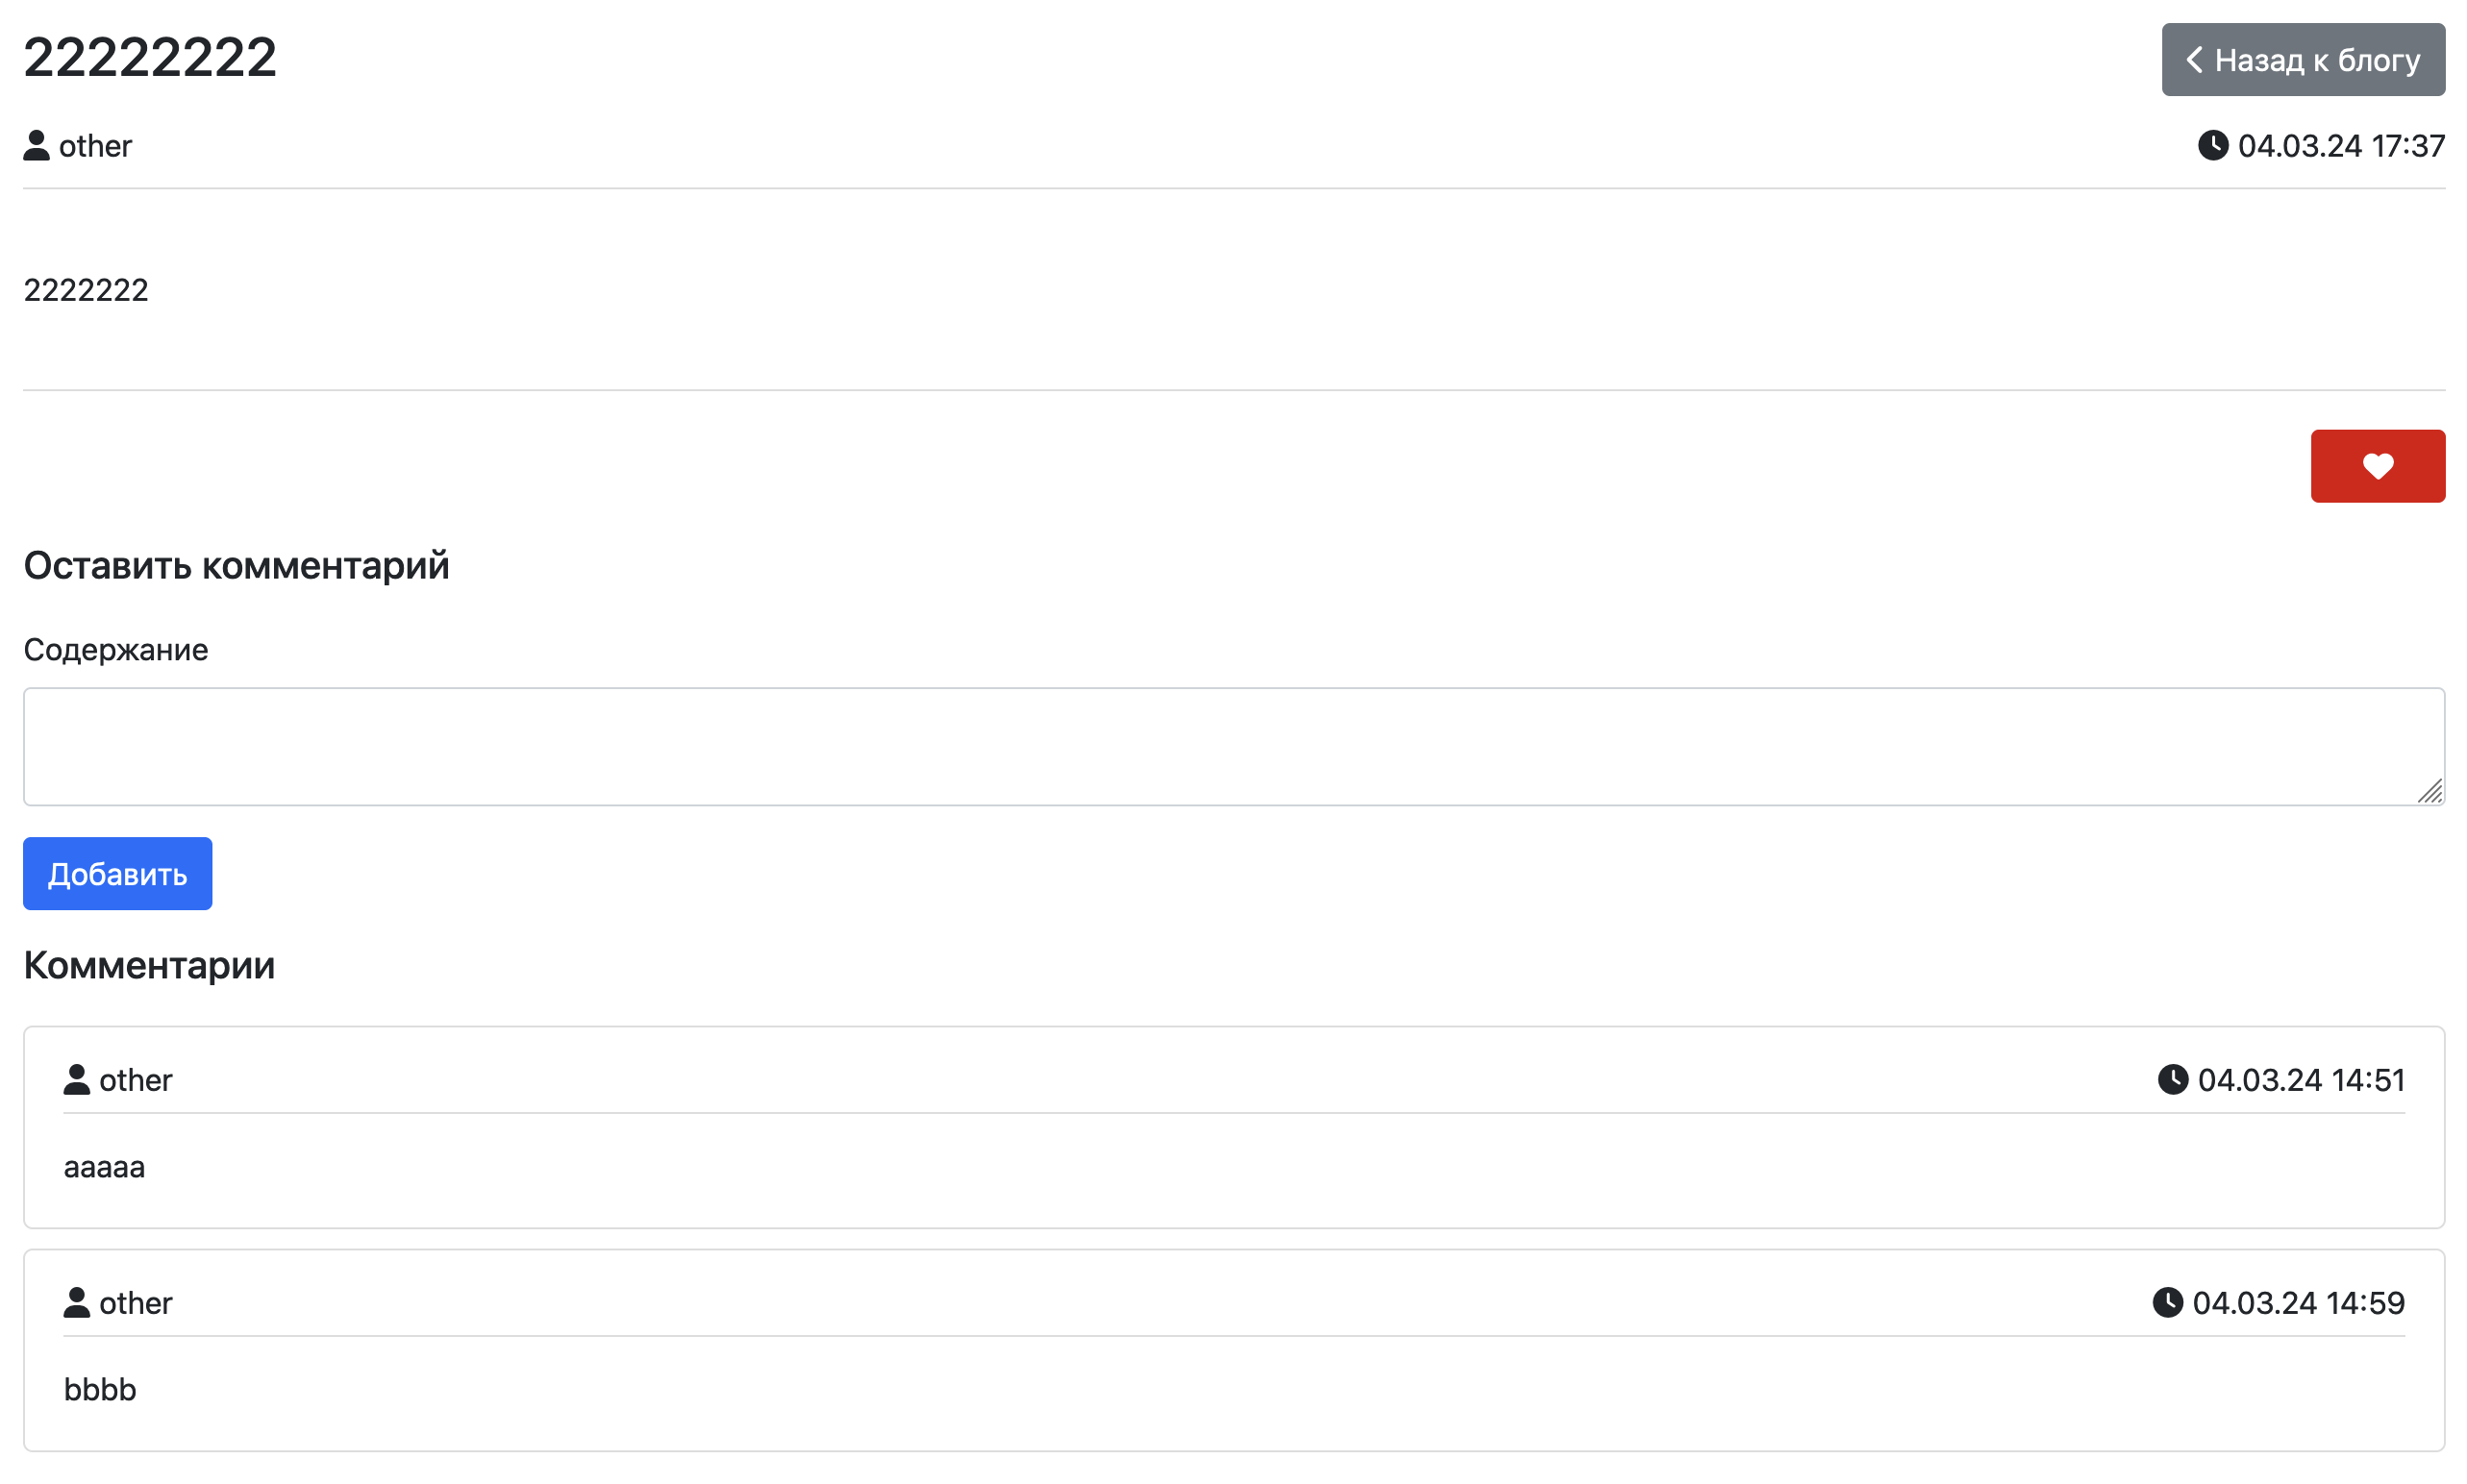
\includegraphics[width=0.8\textwidth]{images/post.png}}
  \caption{Страница, отображаемая при выборе определенного поста}
  \label{fig:post.png}
\end{figure}

\newpage

\section{Вывод}

В ходе выполнения лабораторной работы было разработанное серверное
веб-приложение, отвечающее всем описанным требованиям.

\end{document}
